\section{Оператор обнаружения краев Канни}
Оператор обнаружения краев Канни был разработан Джоном Ф. Канни в 1986 году и использует многоступенчатый алгоритм для выявления различных типов краев на изображении.

\subsection{Разработка алгоритма}
Цель Канни была в том, чтобы найти оптимальный алгоритм обнаружения краев. В данном случае, под ``оптимальным'' имеется в виду следующее:
\begin{enumerate}
  \item хорошее обнаружение --- алгортим должен пометить как можно больше действительных краев на изображении;
  \item хорошая локализация --- помеченные края должны быть близки к действительным насколько это возможно;
  \item минимальный отклик --- каждое ребро должно быть помечено на изображении только один раз, и, где это возможно, шум на изображении не должен быть помечен как края.
\end{enumerate}

Чтобы удовлетворить этим требованиям, Канни использовал вариационное исчисление, которое позволяет найти функцию, которая оптимизирует данный функционал. В операторе обнаружения краев Канни оптимальное функцией является сумма четырех показательных функций. Она может быть аппроксимирована первой производной функции Гаусса.

\subsection{Этапы алгоритма}
\subsubsection{Подавление шума}
В операторе обнаружения краев Канни используется фильтр, в основе которого лежит первая производная функции Гаусса, так как он (фильтр) чувствителен к шуму, присутствующему в необработанном изображении. Поэтому вначале производится свертка изображения с фильтром Гаусса. В результате получается слегка размытое изображение, которое не зависит ни от одного пикселя шума в какой-либо значительной степени.

\begin{figure}
  \centering
  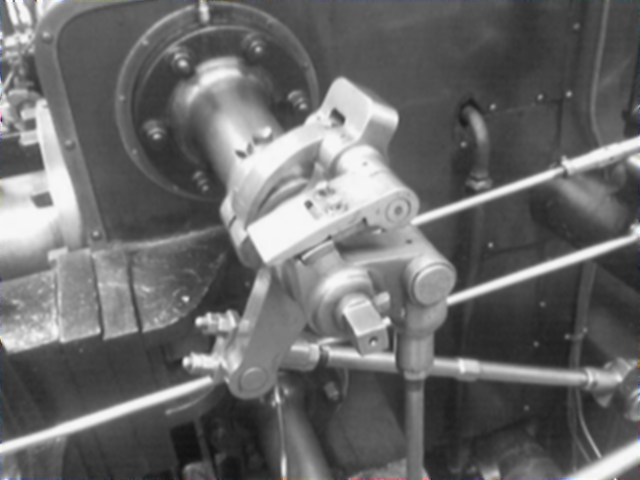
\includegraphics[width=0.9\textwidth]{images/canny-gaussian.png}
  \caption{Изображение после свертки с 5x5-фильтром Гаусса\label{canny-gaussian}}
\end{figure}

Вот пример 5x5 фильтра Гаусса, который используется для размытия изображения $A$, с $\sigma = 1,4$:
\begin{displaymath}
  B = \frac{1}{159}
  \begin{bmatrix}
    2 &  4 &  5 &  4 & 2 \\
    4 &  9 & 12 &  9 & 4 \\
    5 & 12 & 15 & 12 & 5 \\
    4 &  9 & 12 &  9 & 4 \\
    2 &  4 &  5 &  4 & 2
  \end{bmatrix} * A.
\end{displaymath}

\subsubsection{Нахождение градиента интенсивности изображения}
Край на изображении может быть расположен в различных направлениях, поэтому в операторе обнаружения краев Канни используются четыре фильтра для того, чтобы определять горизонтальные, вертикальные и диагональные края в размытом изображении. Каждые оператор обнаружения краев (например, перекрёстный оператор Робертса, Превитт или оператор Собеля) возвращает значения первой производной в горизонтальном направлении $G_y$ и вертикальном направлении $G_x$. Из них могут быть определены градиент и направление края:
\begin{gather*}
  G = \sqrt{G_x^2 + G_y^2},\\
  \Theta = \arctan{\frac{G_y}{G_x}}.
\end{gather*}

\begin{figure}
  \centering
  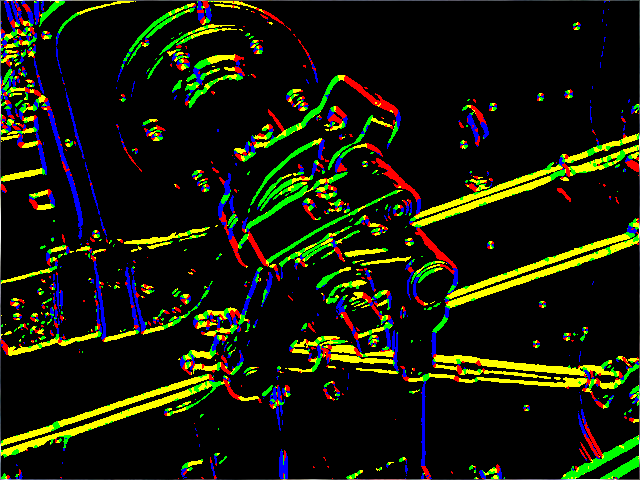
\includegraphics[width=0.9\textwidth]{images/canny-sobel.png}
  \caption{Бинарная карта краев, сделанная с помощью оператора Собеля с порогом равным $80$. Края разукрашены в зависимости от их направленности: желтый для $0^{\circ}$, синий для $90^{\circ}$, зеленый для $45^{\circ}$ и красный для $135^{\circ}$\label{canny-sobel}}
\end{figure}

Угол направленности округляется до одного из четырех значений, представляющих вертикальный, горизонтальный и два диагональных углы ($0$, $45$, $90$ и $135$ градусов, например).

\subsubsection{Подавление немаксимальных значений}
С учетом оценок градиентов изображения, поиск затем производится для определения, предполагает ли величина градиента локальный максимум в его направлении. Например:
\begin{itemize}
  \item если округленный угол равен нулю, то предполагается, что точка находится на краю, если ее интенсивность больше, чем интенсивности в северном и южном направлениях;
  \item если округленный угол равен 90 градусам, то предполагается, что точка находится на краю, если ее интенсивность больше, чем интенсивности в западном и восточном направлениях;
  \item если округленный угол равен 135 градусам, то предполагается, что точка находится на краю, если ее интенсивность больше, чем интенсивности в северо-восточном и юго-западном направлениях;
  \item если округленный угол равен 45 градусам, то предполагается, что точка находится на краю, если ее интенсивность больше, чем интенсивности в северо-западном и юго-восточном направлениях.
\end{itemize}

\begin{figure}
  \centering
  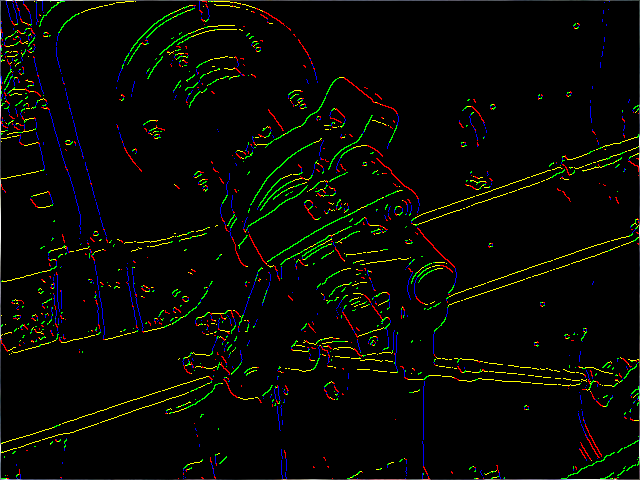
\includegraphics[width=0.8\textwidth]{images/canny-suppression.png}
  \caption{Та же самая бинарная карта, но уже после подавления немаксимальных значений. Края все еще разукрашены для обозначения направленности\label{canny-suppression}}
\end{figure}

На этом этапе мы имеем множество точек краев в форме \emph{бинарного} изображения.

\subsubsection{Отслеживание краев на изображении и определение порога}
Градиенты интенсивности, величина которых велика, вероятнее соответствуют краям на изображении по сравнению с теми, величина которых мала. В большинстве случаев невозможно установить порог (\emph{threshold}), который позволяет отличить край от не края. Поэтому Канни изпользовал установление порога с гистеризисом.

Установление порога с гистеризисом требует два порога --- высокий и низкий. Предположение, что края, представляющие интерес, должны представлять собой непрерывные кривые, позволяет не учитывать те пиксели, которые имеют высокие значения градиента, но не находятся на линии. Следовательно, мы начинаем с применения высокого порога. Это действие помечает края, которые с высокой степенью уверенности можно отнести к действительным. Используя информацию о направлениях, полученную ранее, края на изображении могут быть отслежены. Во время ослеживания края, мы применяем низкий порог, что позволяет отслеживать тусклые части краев, когда мы в состоянии найти начальную точку.

Как только это процесс завершен, мы имеем бинарное изображении, на котором каждый пиксель помечен как принадлежащий какому-либо краю или нет.

\begin{figure}
  \centering
  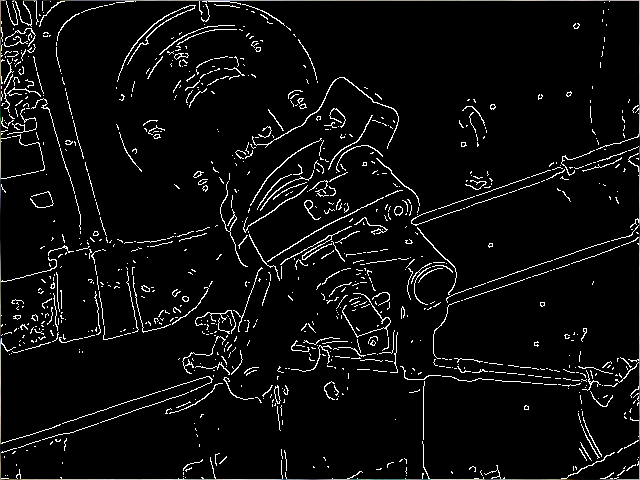
\includegraphics[width=0.8\textwidth]{images/canny-result.png}
  \caption{Изображение парового двигателя после применения оператора обнаружения краев Канни\label{canny-result}}
\end{figure}

\subsection{Параметры алгоритма}
В алгоритме Канни есть несколько регулируемых параметров, которые влияют на время вычислений и эффективность алгоритма.
\begin{itemize}
  \item Размер фильтра Гаусса: сглаживающий фильтр, используемый на первом этапе алгоритма, непосредственно влияет на результат детектора Канни. Меньшие фильтры меньше размывают изображение и позволяют определять мелкие, резкие края. Большие фильтры больше размывают изображение. Большие фильтры целесообразно использовать для определения больших, плавных краев, например, края радуги.
  \item Пороги: использование двух порогов с гистеризисом делает детектор более гибким, чем детекторы с одним пороговым значением. Но несмотря на это, общие проблемы пороговой классификации все еще имеют место быть. При слишком высоком пороге может быть утеряна важная информация. С другой стороны, при слишком низком пороге может быть ошибочно помечена несущественная информация, например, шум.
\end{itemize}

\subsection{Выводы}
Оператор обнаружения краев Канни легко приспосабливаем к различным условиям и требованиям. Его параметризация позволяет использовать его для распознавания краев различного характера.

\newpage
